I dati sono stati raccolti durante diverse giornate utilizzando due diverse configurazioni. Le due configurazioni differiscono per la presenza e l'assenza dell'attenuatore in piombo posto nella parte superiore della cascata dei rivelatori. Il piombo è stato inserito in modo tale da studiare la vita media dei muoni eliminando ulteriormente gran parte dei muoni negativi che tendono a diminuire la vita media e quindi, come si potrà osservare dai risultati, a popolare la parte iniziale dell'istogramma con più dati.
\subsection{Senza Attenuatore}
Nella prima configurazione sperimentale non è stato utilizzato alcun attenuatore in piombo. Durante il periodo di acquisizione, che si è esteso su diversi giorni, sono stati rilevati e misurati un totale di 759 muoni. Tuttavia, il processo di raccolta dei dati ha incontrato diverse difficoltà tecniche, in particolare problemi relativi ai cavi di collegamento tra i vari stadi del circuito logico. Questi cavi tendevano a cessare di funzionare dopo un certo periodo di operatività, richiedendo frequenti sostituzioni. Ciò ha imposto la necessità di un monitoraggio continuo della misura per più giorni, al fine di riavviare la raccolta dei dati in caso di interruzioni inattese. 

Una volta raccolti i dati, è stata eseguita un'analisi tramite ROOT. I dati sono stati organizzati in un istogramma con intervalli (bin) di ampiezza pari a circa $0.1724\mu\mathrm{s}$. Questa scelta rappresenta un compromesso tra la risoluzione temporale del circuito e la quantità di dati raccolti, la quale risultava insufficiente per un'analisi con bin più stretti. L'istogramma è stato quindi sottoposto a un'operazione di fitting utilizzando una funzione esponenziale semplice.
\begin{equation}
    N(t)=Ae^{-\frac{t}{\tau}}
\end{equation}
 %IMMAGINE Muone
\begin{figure}[htp!]
  \centering
  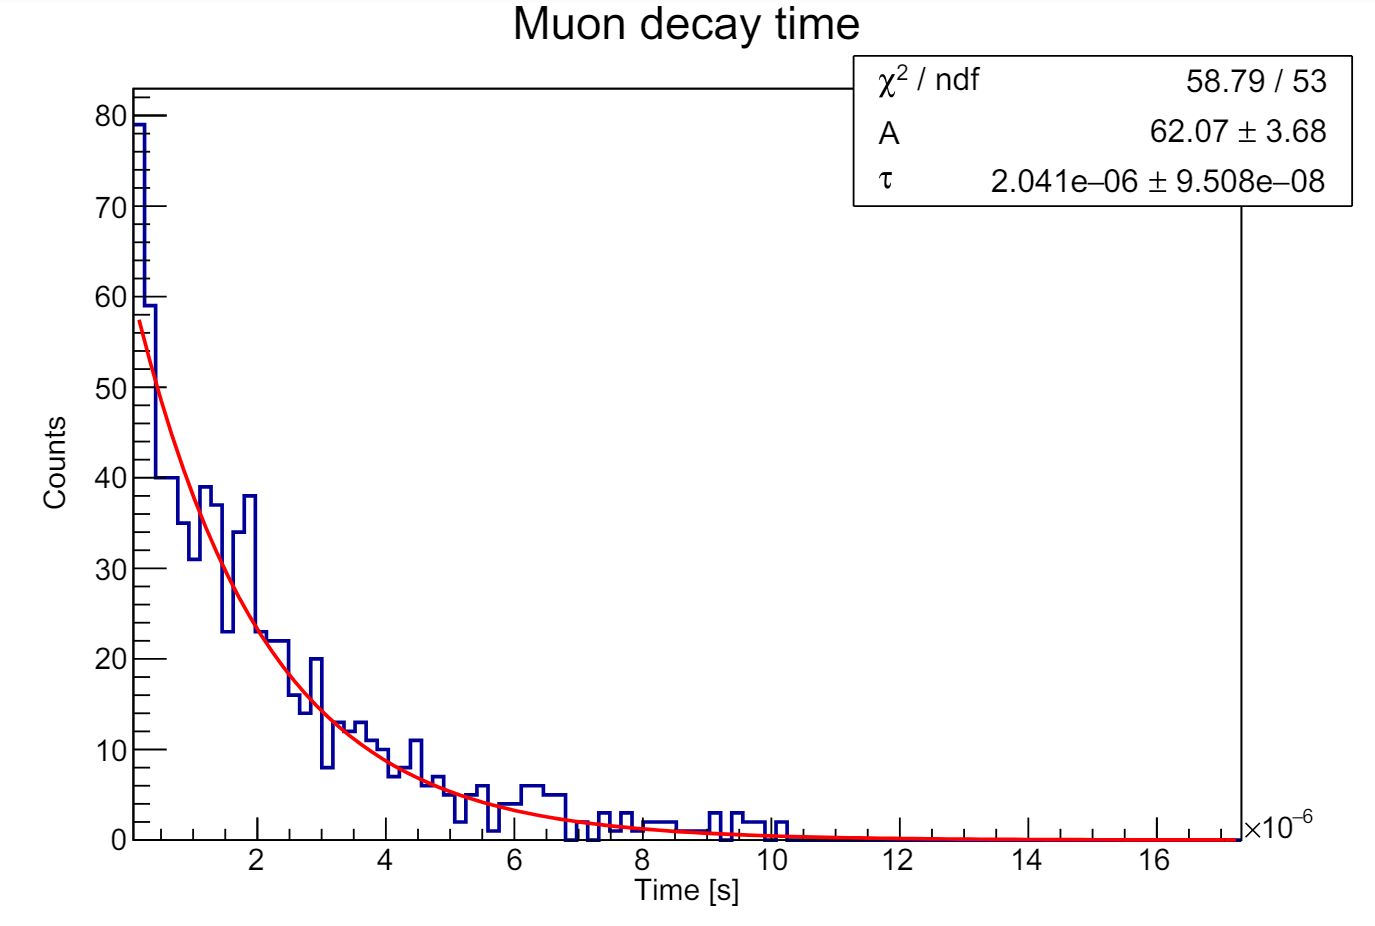
\includegraphics[scale=0.5]{Analisi Dati/MuoniBelli.png} 
  \caption{Questo grafico rappresenta la misura di 759 muoni fermati in un assorbitore in ottone in cui è stato effettuato un fit esponenziale}
\end{figure}
I risultati sono riportati nella tabella \ref{tab:muoni}. 
\begin{table}[H]
    \centering
    \begin{tabular}{| c c c c|}
    \hline
     $\chi^2$ & $ndf$ & Probabilità  & $\tau$ [$\mu s$]\\ [0.5ex] 
 \hline\hline
 58.79& 53 & 27.18 \% & $2.0407\pm0.0096$ \\ 
 \hline
    \end{tabular}
    \caption{Risultatati del fit esponenziale.}
    \label{tab:muoni}
\end{table}
Dato che l'incertezza della vita media data dal fit esponenziale risulta essere più piccola della larghezza dei bin è stato deciso di utilizzare quest'ultima come errore.
\begin{equation}
    \tau_\mu=(2.0407\pm0.1724)\,\mu\unit{s}
\end{equation}
Per valutare qualitativamente il risultato di questa misura si può calcolare di quante sigma si discosta dal  valore teorico. Avendo un'incertezza trascurabile rispetto all'incertezza del nostro esperimento, trattandola come misura di riferimento possiamo assumere che $\sigma_\text{teo}\approx0$. Quindi la discrepanza tra le due misure risulta essere:
\begin{equation}
    \Delta\tau=|\tau_\text{mis}-\tau_\text{teo}|=0.1562\mu\unit{s}
\end{equation}
Dove $\tau_\text{teo} =2.1969\mu\unit{s}$\footnote{Dati ottenuti dal PDG: \url{https://pdg.lbl.gov/index.html}} è la vita media teorica mentre $\tau_\text{mis}$ è la vita media sperimentale. Ora è possibile calcolare di quante $\sigma$ il valore misurato si discosta dal valore teorico.
\begin{equation}
    \Delta \sigma=\frac{\Delta\tau}{\sigma}=0.9
\end{equation}
Di conseguenza la misura si discosta dal valore di riferimento di circa $0.9\sigma$. Questo implica che la vita media misurata per il muone è in buon accordo con il valore atteso.

Un aspetto importante da notare è come i bin iniziali siano molto popolati rispetto agli altri. Questo potrebbe essere dovuto alla presenza dei muoni negativi che attraverso le interazioni con i nuclei degli atomi vengono catturati riducendo così la loro vita media. Per verificare la correttezza di questa ipotesi abbiamo eseguito un secondo esperimento con gli attenuatori in piombo. 
\subsection{Con attenuatore}
Aggiungendo dei blocchi di piombo nelle guide presenti nella struttura in cui sono stati inseriti i rivelatori è possibile ridurre ulteriormente la presenza dei muoni negativi. Dopo aver raccolto 1857 dati ed eseguito un'analoga analisi dati con una larghezza dei bin che corrisponde a $0.0989\mu\unit{s}$. I risultati sono presentati nella tabella \ref{tab:piombo}.
 %IMMAGINE MuonePb
\begin{figure}[htp!]
  \centering
  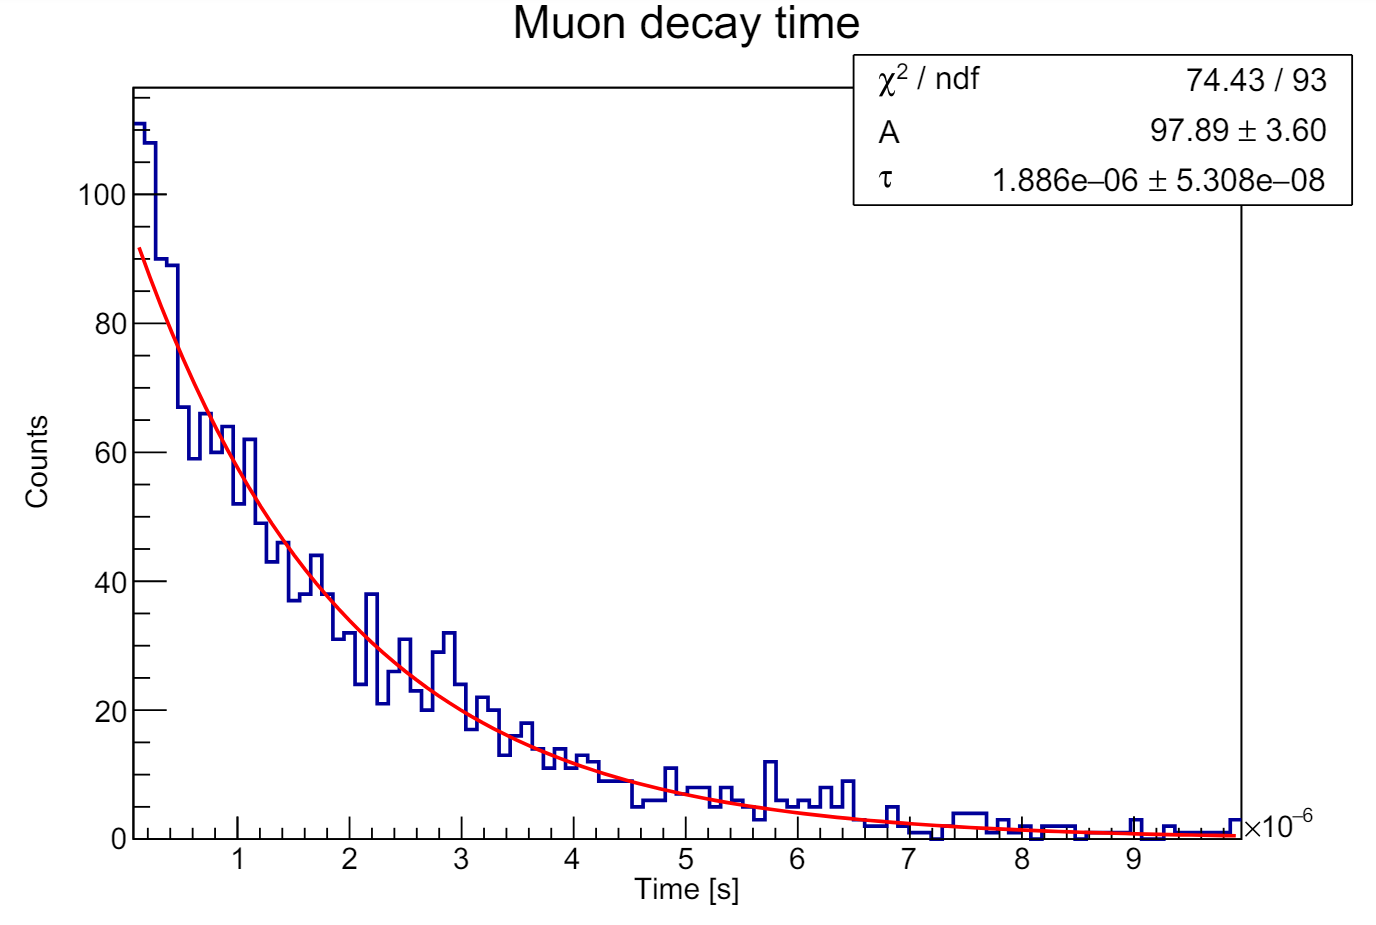
\includegraphics[scale=0.5]{Analisi Dati/MuoniBelliPb.png} 
  \caption{Questo grafico rappresenta la misura di 1857 muoni in cui è stato effettuato un fit esponenziale}
\end{figure}
\begin{table}[H]
    \centering
    \begin{tabular}{| c c c c|}
    \hline
     $\chi^2$ & $ndf$ & Probabilità  & $\tau$ [$\mu s$]\\ [0.5ex] 
 \hline\hline
 74.43 & 93 & 92.14 \% & $1.8857\pm0.0053$ \\ 
 \hline
    \end{tabular}
    \caption{Risultatati del fit esponenziale.}
    \label{tab:piombo}
\end{table}
Dato che l'errore associato alla vita media legato al fit ottenuto è di gran lunga più piccolo della larghezza dei bin del grafico si è optato di scegliere come errore la larghezza del bin stesso. Quindi il risultato di questa misura risulta essere
\begin{equation}
    \tau=(1.8857\pm0.0989)\mu\unit{s}
\end{equation}
Svolgendo un'analoga analisi qualitativa del risultato ottenuto si ottiene che la misura si discosta dal valore teorico di $3.15\sigma$. Questa differenza suggerisce la presenza di effetti sistematici o fenomeni fisici associati all’uso di piombo che alterano la misura. Oltre a questo, l'intera presa dati è stata continua senza essere mai interrotta. Di conseguenza, l’insolita affidabilità dell’apparato sperimentale durante la raccolta dati, sebbene sembri un vantaggio, potrebbe aver introdotto errori sistematici legati alla lunga durata della presa dati senza interruzioni.
